\documentclass{article}
\usepackage{fancyhdr}
\usepackage{graphicx}
\usepackage{amsmath}
\usepackage[margin=1in]{geometry}

\pagestyle{fancy}
\graphicspath{ {./img/} }

\begin{document}
	\begin{titlepage}
		\begin{center}
			\vspace{1cm}
			{\LARGE\textbf{Processing System Circuit}}

			\vspace{1.5cm}
			\textbf{\large Ghassan Arnouk}\\
			
			\vspace{1cm}
			\large SYSC 3006A\\
			\large Summer 2020\\
			\large Lab 2 Report\\
			\large Group 1\\
			
						
			\vspace{2cm}
			\textbf{Instructor:} Michel Sayde\\
			
			\vspace{0.1cm}
			\textbf{TA:} Khalid Almahrog\\
			
			\vspace{0.1cm}
			\textbf{Submitted:} 2020/05/22\\			
		\end{center}
	\end{titlepage}
	
	\lhead{Ghassan Arnouk (Group 1)}
	\rhead{Processing System Circuit}
	\pagebreak
	
	\section{Simple Processing System Circuit}
	\subsection{Discussion Questions}
	\subsubsection {In your own words, describe how SEL and LD are used to control Read and Write operations on the RAM.}
	
	The \textbf{SEL} pin enables or disables the entire RAM module, based on whether the value is 1,floating, or 0. The input is meant primarily ofr situations where you have multiple RAM units, only one of which would be enabled at any time.
	\begin{itemize}
		\item If 0 is inputted, the RAM is disabled
		\item If 1 is inputted, the RAM is enabled
		\item If floating is inputted, the RAM is also enabled\\
	\end{itemize}	
	The \textbf{LD} pin selectes whether the RAM should emit (on \textit{D}) the value at the current address (\textit{A}).
	\begin{itemize}
		\item If 0 is inputted, the RAM (writes) does not emit the value on the \textit{D}
		\item If 1 is inputted, the RAM (reads) emits the value on the \textit{D}
		\item If floating is inputted, the RAM also (reads) emits the value on the \textit{D}\\
	\end{itemize}
	
	\subsubsection {Then based on your observations from 1-1 (a), design and implement some simple logic using only a few logic Gates to interface the WordR and WordW signals from the Control FSM to the SEL and LD signals to implement Read and Write operations. Show a screenshot of your design here.}
	
	\begin{figure}[!htb]
		\centering
		\includegraphics{RAM_circuit.png}
		\caption {RAM Circuit Implementation} 
	\end{figure}
	
	\subsection{Circuit Wiring}
	\begin{center}
	\includegraphics[width=\linewidth]{simple_processing_system_circuit.png}
	\end{center}

	\begin{figure}[h]
		\centering
		\caption {Simple Processing System Circuit}
	\end{figure}	

	\begin{itemize}
		\item Each FSM contains four states: E0 (00), E1 (01), E2 (10), and E3 (11). The output for each state contains a total of 16 bits
		
		\begin{table}[h]
			\centering
			\caption{Information contained within the 16 bits}
			\vspace{0.2cm}
			\begin{tabular}{|c|c|c|}
				\hline
				OPR & 4 bits & ALU operation code\\
				\hline
				Reg & 4 bits & Register address\\
				\hline
				WordR & 1 bit & Word read enable\\
				\hline
				WordW & 1 bit & Word write enable\\
				\hline
				T1OE & 1 bit & T1 output enable (read)\\
				\hline
				T1CE & 1 bit & T1 clock enable (write)\\
				\hline
				T2OE & 1 bit & T2 output enable (read)\\
				\hline
				T2CE & 1 bit & T2 clock enable (write)\\
				\hline
				Next State & 2 bits & Next State\\
				\hline				
			\end{tabular}
		\end{table}
	
	\item Note that the information is written in hexadecimal notation
	\end{itemize}

	\pagebreak
	
	\subsection{ROM FSMs}
	
		\subsubsection{Fill in a next state table (ROM table) for the following RTL.}
		\begin{table}[!h]
			\centering
			\caption{R10 $\leftarrow$ R1 OR R2}
			\vspace{0.2cm}
			\begin{tabular}{|c|c|c|c|c|c|c|c|c|c|c|}
				\hline
				State & OPR (4 bits) & Reg (4 bits) & WordR & WordW & T1CE & T1OE & T2CE & T2OE & Next State & Hex\\
				\hline\hline
				E0=00 & 0000 & 0001 & 1 & 0 & 1 & 0 & 0 & 0 & 01 & 01A1\\
				\hline
				E1=01 & 0001 & 0010 & 1 & 0 & 0 & 1 & 1 & 0 & 10 & 529A\\
				\hline
				E2=10 & 0000 & 1010 & 0 & 1 & 0 & 0 & 0 & 1 & 00 & 0A44\\
				\hline
			\end{tabular}
		\end{table}		

		\subsubsection{Fill in a next state table (ROM table) for the following RTL.}
		\begin{table}[h]
			\centering
			\caption{R11 $\leftarrow$ R2 - R10}
			\vspace{0.2cm}
			\begin{tabular}{|c|c|c|c|c|c|c|c|c|c|c|}
				\hline
				State & OPR (4 bits) & Reg (4 bits) & WordR & WordW & T1CE & T1OE & T2CE & T2OE & Next State & Hex\\
				\hline\hline
				E0=00 & 0000 & 0010 & 1 & 0 & 1 & 0 & 0 & 0 & 01 & 02A1\\
				\hline
				E1=01 & 0010 & 1010 & 1 & 0 & 0 & 1 & 1 & 0 & 10 & 2A9A\\
				\hline
				E2=10 & 0000 & 1011 & 0 & 1 & 0 & 0 & 0 & 1 & 00 & 0B44\\
				\hline
			\end{tabular}
		\end{table}

		\subsubsection{Fill in a next state table (ROM table) for the following RTL.}
		\begin{table}[h]
			\centering
			\caption{R12 $\leftarrow$ NOT(R11)}
			\vspace{0.2cm}
			\begin{tabular}{|c|c|c|c|c|c|c|c|c|c|c|}
				\hline
				State & OPR (4 bits) & Reg (4 bits) & WordR & WordW & T1CE & T1OE & T2CE & T2OE & Next State & Hex\\
				\hline\hline
				E0=00 & d & d & d & d & d & d & d & d & 01 & 0001\\
				\hline
				E1=01 & 0111 & 1011 & 1 & 0 & 0 & 1 & 1 & 0 & 10 & 7B9A\\
				\hline
				E2=10 & 0000 & 1100 & 0 & 1 & 0 & 0 & 0 & 1 & 00 & 0C44\\
				\hline
			\end{tabular}			
		\end{table}
	
		\subsubsection{Fill in a next state table (ROM table) for the following RTL.}
		\begin{table}[!h]
			\centering
			\caption{R13 $\leftarrow$ R0 + R12}
			\vspace{0.2cm}		 
			\begin{tabular}{|c|c|c|c|c|c|c|c|c|c|c|}
				\hline
				State & OPR (4 bits) & Reg (4 bits) & WordR & WordW & T1CE & T1OE & T2CE & T2OE & Next State & Hex\\
				\hline\hline
				E0=00 & 0000 & 0000 & 1 & 0 & 1 & 0 & 0 & 0 & 01 & 00A1\\
				\hline
				E1=01 & 0001 & 1100 & 1 & 0 & 0 & 1 & 1 & 0 & 10 & 1C9A\\
				\hline
				E2=10 & 0000 & 1101 & 0 & 1 & 0 & 0 & 0 & 1 & 00 & 0D44\\
				\hline
			\end{tabular}
		\end{table}
		
		\pagebreak
		
		\subsection{Execute the first RTL starting at state E0 and finishing at state E2. Do the same for the rest and observe their execution to make sure that there is no errors.}
		
		\subsubsection{After finishing all executions, Log the execution of the sequence on your implementation and show the results here.}		
		\begin{table}[!ht]
			\centering
			\caption{Simulation Log of the Simple Processing Circuit}
			\vspace{0.2cm}
			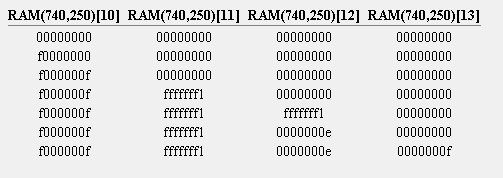
\includegraphics[width=0.8\linewidth]{log_sim_table_part1.png}
		\end{table}
	
		\subsubsection{After the executions of R11 ← R2 – R10, what is the value of R11 (in decimal)?}
		The value of R11 in decimal after the executions is 4294967281. The decimal from signed 2's complement is -15.
		
		\subsubsection{What does the operations R12 ← NOT (R11) and R13 ← R0 + R12 accomplish (think about what does the value obtained in R13 represent in relation to R11 and R12, and why)?}
		R12 is the 2's complement of R11. Furthermore, fffffff1 (-14) is the 2's complement of 0000000e (14).
		R13 is the sum of R0 and R12. Adding 00000001 (1) to 0000000e (14) will result in 0000000f (15).
		
		\pagebreak
		
		\section{Generalized Processing System Circuit}
		
		\subsection{Circuit Wiring}
		\begin{figure}[!h]
			\centering
			\includegraphics[width=\linewidth]{generalized_processing_system_circuit.png}
			\caption{Generalized Processing System Circuit}
		\end{figure}

		\subsection{Complete the following next state table for the Control FSM that executes every instruction.}
		\begin{table}[!h]
			\centering
			\setlength\tabcolsep{2pt}
			\caption{Control FSM}
			\vspace{0.2cm}	 
			\begin{tabular}{|c|c|c|c|c|c|c|c|c|c|c|c|c|c|}
				\hline
				State (ROM) Adress & AOP & ANOP & DR & SXR & SYR & WordR & WordW & T1CE & T1OE & T2CE & T2OE & Next State & Inst.(Hex)\\
				\hline\hline
				(D)=00 & 0 & 1 & 0 & 0 & 0 & 0 & 0 & 0 & 0 & 0 & 0 & 00 & 0801\\
				\hline
				(E0)=00 & 0 & 1 & 0 & 1 & 0 & 1 & 0 & 1 & 0 & 0 & 0 & 10 & 0AA2\\
				\hline
				(E1)=01 & 1 & 0 & 0 & 0 & 1 & 1 & 0 & 0 & 1 & 1 & 0 & 11 & 119B\\
				\hline
				(E2)=10 & 0 & 1 & 1 & 0 & 0 & 0 & 1 & 0 & 0 & 0 & 1 & 00 & 0C44\\
				\hline
			\end{tabular}
		\end{table}

		\pagebreak

		\subsection{Complete the Encoded Instruction Table for same 4 instructions of the Part I of this lab.}
		\begin{table}[!h]
			\centering
			\caption{Encoded Instruction}
			\vspace{0.2cm}		 
			\begin{tabular}{|c|c|c|}
				\hline
				Operation & Encoded 16-bit Value (in Binary) & Encoded 16-bit Value (in Hex)\\
				\hline\hline
				R10 $\leftarrow$ R1 OR R2 & 0b: 0101 1010 0001 0010 & 5A12\\
				\hline
				R11 $\leftarrow$ R2 - R10 & 0b: 0010 1011 0010 1010 & 2B2A\\
				\hline
				R12 $\leftarrow$ NOT(R11) & 0b: 0111 1100 0000 1011 & 7C0B\\
				\hline
				R13 $\leftarrow$ R0 + R12 & 0b: 0001 1101 0000 1100 & 1D0C\\
				\hline
			\end{tabular}
		\end{table}
	
		\subsection{To execute the first operation, poke its 16-bit encoder value into IR, and then poke the Toggle Switch to advance the FSM through the operation. Do the same for the rest and observe their execution to make sure that there is no errors.}
		
		\subsubsection{After finishing all executions, Log the execution of the sequence on your implementation and show the results here.}
		\begin{table}[!ht]
			\centering
			\caption{Simulation Log of the Generalized Processing Circuit}
			\vspace{0.2cm}
			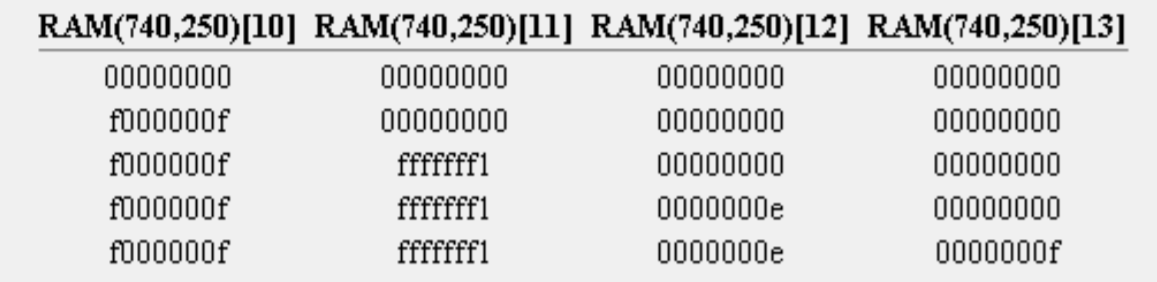
\includegraphics[width=0.8\linewidth]{log_sim_table_part2.png}			
		\end{table}
		
		\subsubsection{Compare the results obtained here to Part I, they should be same. So, what is the advantage of the generalized machine in part II (here) over the simple machine of part I (above)?}
		The generalized processing system circuit is a lot more quicker as it allows the user to do multiple ALU operations without having to change the instructions in the ROM-based FSM. In the simple machine, each operation involving the ALU requires a unique FSM table. However, the generalized machine is implemented such that it encodes the differences among operations in a way that can be manipulated by the FSM.
\end{document}